\documentclass[english,14pt]{beamer}
\usetheme{EastLansing}
\usecolortheme{spruce}

\usepackage{xcolor}
\usepackage{listings}
\usepackage{courier}
\usepackage{graphicx}
\usepackage{amsmath}
\usepackage{algorithm2e}
\usepackage{multicol}
\usepackage{hyperref}
\usepackage{textcomp}

% http://mirrors.ibiblio.org/CTAN/macros/latex/contrib/datetime2/datetime2.pdf
\usepackage{babel}
\usepackage[useregional]{datetime2}

% https://tex.stackexchange.com/questions/42619/x-mark-to-match-checkmark
\usepackage{pifont}% http://ctan.org/pkg/pifont

%% https://stackoverflow.com/questions/1435837/how-to-remove-footers-of-latex-beamer-templates
%%gets rid of bottom navigation bars
%\setbeamertemplate{footline}[page number]
%
%gets rid of navigation symbols
\setbeamertemplate{navigation symbols}{}


\usefonttheme[onlymath]{serif}

\definecolor{mGreen}{rgb}{0,0.6,0}
\definecolor{mGray}{rgb}{0.5,0.5,0.5}
\definecolor{mPurple}{rgb}{0.8,0,0.82}
\definecolor{backgroundColour}{rgb}{0.95,0.95,0.92}
\definecolor{lightBlue}{rgb}{0.1, 0.1, 0.8}
\definecolor{darkGreen}{rgb}{0, 0.39, 0}

\newcommand\red[1]{{\color{red} #1}}
\newcommand\green[1]{{\color{green} #1}}
\newcommand\blue[1]{{\color{blue} #1}}
\newcommand\darkGreen[1]{{\color{darkGreen} #1}}

\newcommand{\cmark}{\ding{51}}%
\newcommand{\xmark}{\ding{55}}%

\lstdefinestyle{CStyle}{
    backgroundcolor=\color{backgroundColour},   
    commentstyle=\color{mGreen},
    keywordstyle=\color{magenta},
    numberstyle=\tiny\color{mGray},
    stringstyle=\color{mPurple},
    basicstyle=\footnotesize,
    breakatwhitespace=false,         
    breaklines=true,                 
    captionpos=b,                    
    keepspaces=true,                 
    numbers=left,                    
    numbersep=5pt,                  
    showspaces=false,                
    showstringspaces=false,
    showtabs=false,                  
    tabsize=2,
    language=Python
}

\lstdefinestyle{pseudo}{
        basicstyle=\ttfamily\footnotesize,
        keywordstyle=\color{lightBlue},
        morekeywords={BEGIN,END,IF,ELSE,ENDIF,ELSEIF,PRINT,WHILE,RETURN,ENDWHILE,DO,FOR,TO,IN,ENDFOR,BREAK,INPUT,CONDITIONS},
        morecomment=[l]{//},
        commentstyle=\color{mGreen}
}

\lstset{basicstyle=\footnotesize\ttfamily,breaklines=true}
\lstset{framextopmargin=50pt,tabsize=2}

\title{ENGG1003 - Thursday Week 9}
\subtitle{Random numbers from normal distributions \\
---aka random numbers from Gaussian distributions}
\author{Steve Weller}
\institute{University of Newcastle}
%\date{\today}
\date{6 May 2021}

% following is a bit of a hack, but forces page numbers (technically: frame numbers) to run 1,2,3,... 
% with titlepage counting as frame 1

\addtocounter{framenumber}{1}
\titlepage

\begin{document}

\begin{flushleft}
{\scriptsize Last compiled:~\DTMnow}
\vspace*{-5mm}
\end{flushleft}
\framebreak

%==============================================================

\begin{frame}[fragile]

\frametitle{Lecture overview}
\begin{enumerate}
%	\item recap: uniformly distributed random numbers
%	\begin{itemize}
%		\item pdf of uniformly distributed rv
%		\item area under pdf is probability
%		\item histogram, normalized histogram is basically pdf
%	\end{itemize}

	\item[]
	
	\item normal distribution
	\begin{itemize}
		\item also known as ``bell curve'', or Gaussian distribution
%		\item today: ``standard'' normal ie: mean $\mu = 0$ and $\sigma = 1$ %zero and std 1, 
		\item today: draw random samples from ``standard'' normal distribution
%		\item histogram
	\end{itemize}
	
	\item[]
	
	\item compute probabilities using normal distribution
	\begin{itemize}
		\item uses numerical integration
	\end{itemize}
	
%	\item[]
%	
%	\item normal distribution (aka Gaussian)
%	\begin{itemize}
%		\item pdf, meaning of $\mu$ and $\sigma$
%		\item generate using Python
%		\item area (needs integration) and probability
%	\end{itemize}
	
%	\item[]
%	
%	\item engineering application
	
\end{enumerate}

\end{frame}

%%==============================================================
%
%\begin{frame}[fragile]
%
%\frametitle{$1)$ Uniformly distributed random numbers}
%
%% https://www.w3schools.com/python/python_ml_data_distribution.asp
%
%\begin{itemize}
%	\item reminder: introduced in week 4
%	\item general form: random.uniform(low=0.0, high=1.0, size=None)
%	\item Create an array containing 250 random floats between 0 and 5
%\end{itemize}
%
%%  random.uniform(low=0.0, high=1.0, size=None)
%
%\texttt{filename.py}
%\begin{lstlisting}[style=CStyle,basicstyle=\scriptsize]
%import numpy as np
%
%x = np.random.uniform(0.0, 5.0, 250)
%
%print(x) 
%\end{lstlisting}
%
%\end{frame}

%%==============================================================
%
%\begin{frame}[fragile]
%
%\frametitle{histogram}
%
%% https://www.w3schools.com/python/matplotlib_histograms.asp
%
%% https://www.w3schools.com/python/python_ml_data_distribution.asp
%
%\begin{itemize}
%	\item A histogram is a graph showing frequency distributions
%	\item It is a graph showing the number of observations within each given interval.
%	\item To visualize the data set we can draw a histogram with the data we collected
%	\item We will use the Python module Matplotlib to draw a histogram
%\end{itemize}
%
%\texttt{filename.py}
%\begin{lstlisting}[style=CStyle,basicstyle=\scriptsize]
%import numpy as np
%import matplotlib.pyplot as plt
%
%x = np.random.uniform(0.0, 5.0, 250)
%
%plt.hist(x, 5)
%plt.show() 
%\end{lstlisting}
%
%\end{frame}

%%==============================================================
%
%\begin{frame}[fragile]
%
%\frametitle{}
%
%\begin{figure}[ht]
%	\centering
%	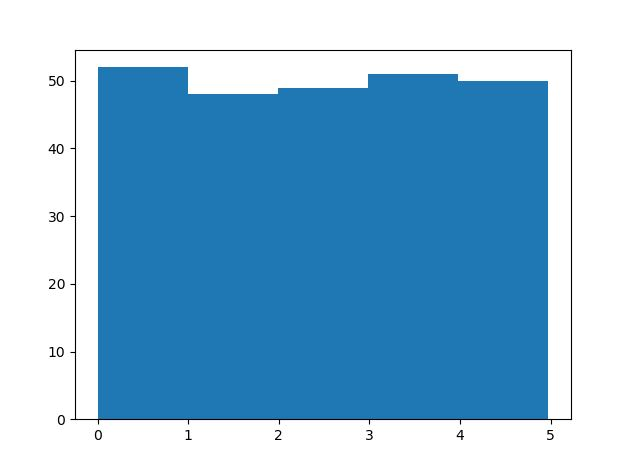
\includegraphics[width=0.8\textwidth]{figures/uniformOutput}
%\end{figure}
%
%\begin{itemize}
%	\item interpret in terms of numbers in each bin
%	\item be clear about bin ranges $[a,b)$
%\end{itemize}
%
%\end{frame}

%%==============================================================
%
%\begin{frame}[fragile]
%
%\frametitle{pdf of uniformly distributed rv}
%
%\begin{itemize}
%	\item probability density function of the uniform distribution is
%	\[
%		p(x) = \frac{1}{b-a}
%	\]
%	anywhere in the interval $[a,b)$, and zero elsewhere
%	\item needs an image
%\end{itemize}
%
%\end{frame}

%%==============================================================
%
%\begin{frame}[fragile]
%
%\frametitle{normalized histogram is basically pdf}
%
%\begin{itemize}
%	\item same plot as previous, but now normalize using \texttt{density=True} in \texttt{hist}
%\end{itemize}
%
%\end{frame}

%%==============================================================
%
%\begin{frame}[fragile]
%
%\frametitle{area under pdf is probability}
%
%\begin{itemize}
%	\item xxx
%\end{itemize}
%
%\end{frame}

%==============================================================

\begin{frame}[fragile]

\frametitle{$1)$ Normal distribution}

\begin{itemize}
	\item intoduced \emph{uniformly} distributed random numbers in week 4
	\item today: will focus on ``standard'' normal, extend next week to general form
	\item goal today is to random samples from a standard normal (Gaussian) distribution, and compute probability of number falling in specified range
	\item aka Gaussian random numbers
	\item widely appear in engineering
\end{itemize}

\end{frame}

%==============================================================

\begin{frame}[fragile]

\frametitle{Standard normal distribution}

\begin{itemize}
	\item Straight into it, generate $100,000$ random numbers generated using \texttt{normal} function in numpy's random library
	\item standard: mean = 0, std = 1
\end{itemize}



\texttt{filename.py}
\begin{lstlisting}[style=CStyle,basicstyle=\scriptsize]
import numpy as np
import matplotlib.pyplot as plt

np.random.seed(1)
x = np.random.normal(0.0, 1.0, size=100000)

plt.hist(x, 10)
plt.show() 
\end{lstlisting}

\end{frame}

%==============================================================

\begin{frame}[fragile]

\frametitle{}

\begin{itemize}
	\item code commentary
	\item normal random numbers aka Gaussian distribution
	\item general form of call to normal()
	\item explain hist()
	\item live demo
	\item nothing much to see in plot of numbers themselves ``noise'' 
\end{itemize}

\end{frame}

%==============================================================

\begin{frame}[fragile]

\frametitle{Histogram}

\begin{itemize}
	\item interpret histogram
	\item bins, counts, examples
	\item call hist to return bins---too hard?
\end{itemize}

\begin{itemize}
	\item A histogram is a graph showing frequency distributions
	\item It is a graph showing the number of observations within each given interval.
	\item To visualize the data set we can draw a histogram with the data we collected
	\item We will use the Python module Matplotlib to draw a histogram
\end{itemize}

\end{frame}

%==============================================================

\begin{frame}[fragile]

\frametitle{Python code}

\texttt{histdemo.py}
\begin{lstlisting}[style=CStyle,basicstyle=\scriptsize]
# histdemo
import numpy as np
import matplotlib.pyplot as plt

np.random.seed(1)
d = np.random.normal(0.0, 1.0, size=100000)

x = np.linspace(-5,5,num=1000)
f = 1/(np.sqrt(2 * np.pi)) * np.exp(-x**2 / 2)

plt.hist(d, 100, density=True)
plt.plot(x, f, color='r', linewidth=3)
#plt.hist(d, 100)

#plt.plot(d, 'o')
plt.show()
\end{lstlisting}

%\begin{itemize}
%	\item lines 5--6: PDF of standard normal distribution
%\end{itemize}

\end{frame}

%==============================================================

\begin{frame}[fragile]

\frametitle{Histogram: 10 bins}

\begin{figure}[ht]
	\centering
	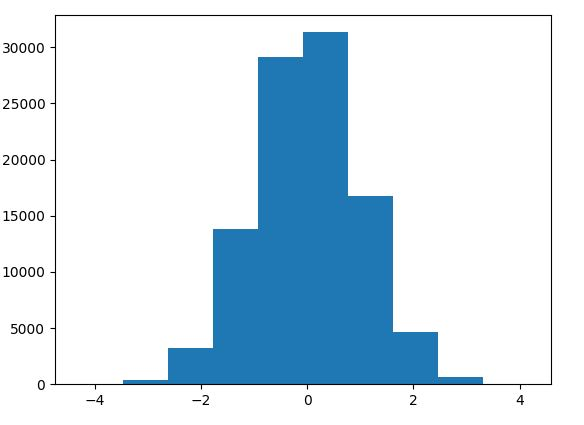
\includegraphics[width=0.7\textwidth]{figures/hist10BinsExample}
\end{figure}

\begin{itemize}
	\item eg: XXX samples in range $[XXX,XXX]$
\end{itemize}

\end{frame}

%==============================================================

\begin{frame}[fragile]

\frametitle{Histogram: 100 bins}

\begin{figure}[ht]
	\centering
	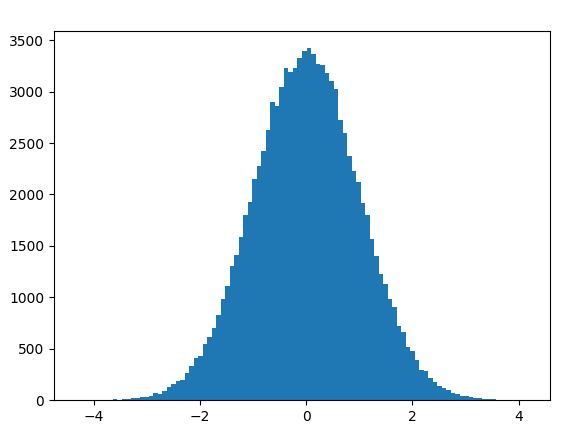
\includegraphics[width=0.7\textwidth]{figures/hist100BinsExample}
\end{figure}

\begin{itemize}
	\item identical data set as for $10$ bins
\end{itemize}

\end{frame}

%==============================================================

\begin{frame}[fragile]

\frametitle{Normalized histogram (area $1$): 100 bins}

\begin{lstlisting}[style=CStyle,basicstyle=\scriptsize]
plt.hist(x, 100, density=True)
\end{lstlisting}

\begin{figure}[ht]
	\centering
	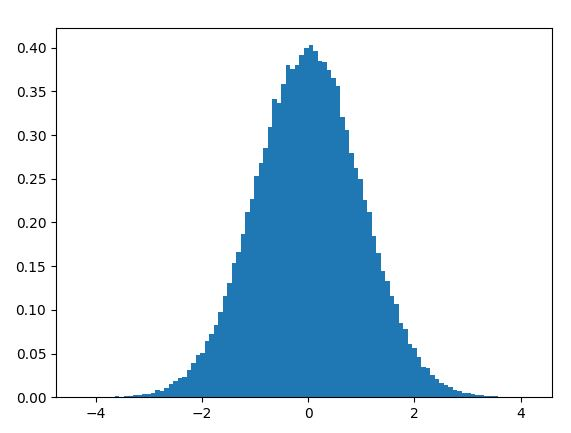
\includegraphics[width=0.7\textwidth]{figures/hist100BinsDensity}
\end{figure}

\end{frame}

%==============================================================

\begin{frame}[fragile]

\frametitle{Normalized histogram with PDF}

\begin{figure}[ht]
	\centering
	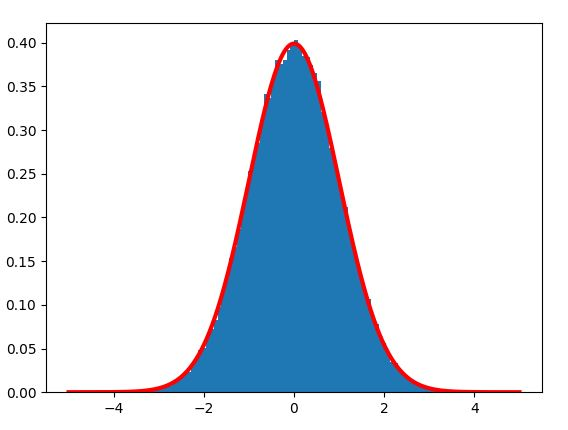
\includegraphics[width=0.7\textwidth]{figures/histWithpdf}
\end{figure}

\begin{itemize}
	\item[] red curve is \red{\emph{probability density function (PDF)}}
\end{itemize}

\end{frame}

%==============================================================

\begin{frame}[fragile]

\frametitle{Standard normal distribution}

Standard normal probability density function:
\[
\boxed{
f(x) = \frac{1}{\sqrt{2\pi}} e^{-x^2/2}}
\]

%\begin{lstlisting}[style=CStyle,basicstyle=\scriptsize]
%import numpy as np
%import matplotlib.pyplot as plt
%
%x = np.linspace(-5,5,num=1000)
%f = 1/(np.sqrt(2 * np.pi)) * np.exp(-x**2 / 2)
%plt.plot(x, f, color='r', linewidth=3)
%\end{lstlisting}

\begin{itemize}
	\item we'll see a more general form of normal distribution next lecture
	\item standard normal is a special case: mean 0 and std 1
	\item reflections
	\item qualitative description of what a pdf is
\end{itemize}

\end{frame}

%==============================================================

\begin{frame}[fragile]

\frametitle{Probability density functions}

If $X$ is a random number drawn from a distribution with PDF $f(x)$, probability $X$ takes a value in interval $[a,b]$ is
\vspace*{-2mm}
\[
	\boxed{
\mathrm{P}(a \leq X \leq b) = \int_a^b f(x) dx}
\]
\vspace*{-5mm}
\begin{figure}[ht]
	\centering
	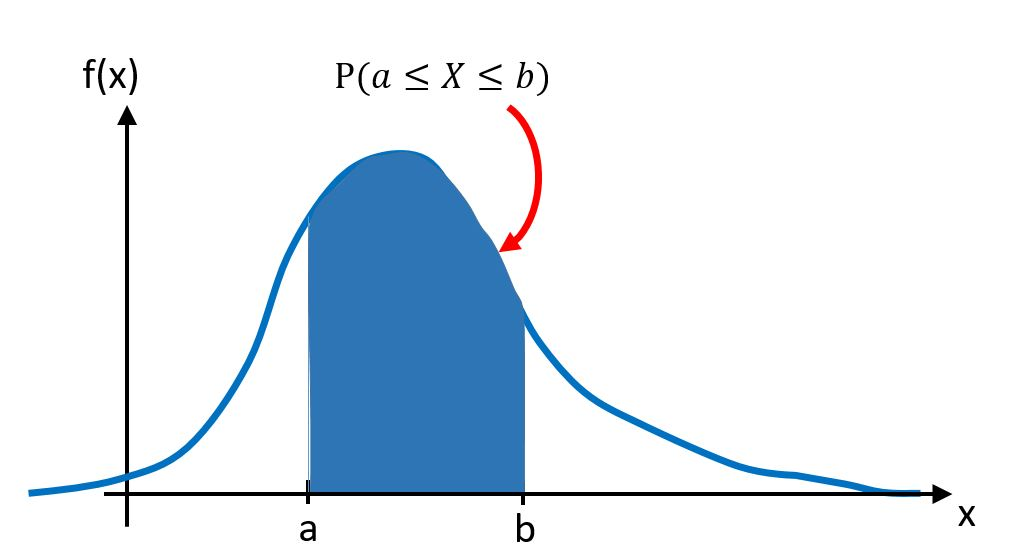
\includegraphics[width=.7\textwidth]{figures/genericPDF}
\end{figure}

\end{frame}

%==============================================================

\begin{frame}[fragile]

\frametitle{Properties of a PDF}

To qualify as a PDF, function $f$ must be non-negative, and must have the normalization property. Thsi means the entire area under the graph of $f$ must be equal to $1$

\begin{itemize}
	\item area under $f(x)$ is $1$
	\begin{itemize}
		\item reason for the $1/\sqrt{2\pi}$ factor
	\end{itemize}
	
	\item[]
	
	\item $f(x) \geq 0$ for all $x$, since probability can't be negative
	
	\item[]
	
	\item total area under pdf is $1$, since $X$ must take some value
\[
\int_{-\infty}^\infty f(x) dx = \mathrm{P}(-\infty \leq X \leq \infty) = 1
\]
\end{itemize}

\end{frame}

%==============================================================

\begin{frame}[fragile]

\frametitle{$2)$ Integration}

the story so far \ldots

\begin{itemize}
	\item PDF of random numbers following \red{\emph{standard normal distribution}} is a ``bell curve''
\[
	f(x) = \frac{1}{\sqrt{2\pi}} e^{-x^2/2}
\]
	\item probability of a random number drawn from standard normal distribution taking value in interval $[a,b]$ is
	\[
	\mathrm{P}(a \leq X \leq b) = \frac{1}{\sqrt{2\pi}} \int_a^b  e^{-x^2/2} dx
	\]

\end{itemize}

\end{frame}

%==============================================================

\begin{frame}[fragile]

\frametitle{Example}

\begin{itemize}
	\item exact expression doesn't exist for $\int_a^b e^{-x^2/2} dx$
	\item need to use numerical integration
\end{itemize}

\textbf{Example}

\begin{itemize}
	\item $a = 1$, $b = 2$
	\item calculated probability using \texttt{standardnormal.py} is $0.1359$
	\begin{itemize}
		\item uses trapezoidal method with $100$ sub-intervals on $[1,2]$
	\end{itemize}
\end{itemize}

\end{frame}

%==============================================================

\begin{frame}[fragile]

\frametitle{}

\begin{figure}[ht]
	\centering
	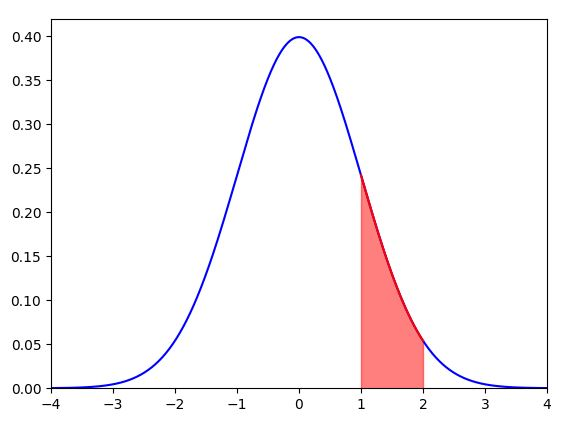
\includegraphics[width=.7\textwidth]{figures/stdnormal_12}
\end{figure}

red shaded area is
\[
\frac{1}{\sqrt{2\pi}} \int_1^2 e^{-x^2/2} dx \approx 0.1359
\]

\end{frame}

%==============================================================

\begin{frame}[fragile]

\frametitle{Python code: fraction of numbers in $[a,b]$}

\texttt{standardnormal.py}
\begin{lstlisting}[style=CStyle,basicstyle=\scriptsize]
# standardnormal
import numpy as np
import matplotlib.pyplot as plt

def f(x):
    return 1/(np.sqrt(2 * np.pi)) * np.exp(-x**2 / 2)

def trapezoidal(f, a, b, n):
    h = (b-a)/n
    f_sum = 0
    for i in range(1, n, 1):
        x = a + i*h
        f_sum = f_sum + f(x)
    return h*(0.5*f(a) + f_sum + 0.5*f(b))
\end{lstlisting}

\begin{itemize}
	\item lines 5--6: PDF of standard normal distribution
\end{itemize}

\end{frame}

%==============================================================

\begin{frame}[fragile]

\frametitle{Python code}

\texttt{standardnormal.py}---continued
\begin{lstlisting}[style=CStyle,basicstyle=\scriptsize]
a = 1
b = 2
prob_ab = trapezoidal(f, a, b, 100)
print('Probability X in range [{},{}] is: {:.4f}'.format(a, b, prob_ab))

x = np.linspace(-4, 4, 1000)
xab = np.linspace(a, b, 100)

plt.plot(x, f(x), 'b')             # standard normal pdf
plt.plot(xab,f(xab),'r')
plt.fill_between(xab,f(xab),color='r',alpha=0.5) #alpha=transparency
plt.axis([-4, 4, 0, 0.42])
plt.show()
\end{lstlisting}

\begin{itemize}
	\item line 3: approximate $\frac{1}{\sqrt{2\pi}} \int_1^2 e^{-x^2/2} dx$
	\item line 7: $1 \leq x \leq 2$ for red shaded area plot
\end{itemize}

\end{frame}

%==============================================================

\begin{frame}[fragile]

\frametitle{Demo of standard normal generation}

\begin{itemize}
	\item generate $10^6$ random numbers
	\item expect $10^6 \times 0.1359 = 135,900$ in range $[1,2]$
	\item live demo
	\item results
\end{itemize}

\end{frame}

%==============================================================

\begin{frame}[fragile]

\frametitle{Python code}

\texttt{standardnormaldemo.py}
\begin{lstlisting}[style=CStyle,basicstyle=\scriptsize]
# standardnormaldemo
import numpy as np

N = 1000000
x = np.random.normal(0.0, 1.0, size=N)
a = 1
b = 2
num_ab = 0
for k in range(0, len(x)):
    if a <= x[k] <= b:
        num_ab += 1

print('{} standard normal random numbers'.format(N))
print('Fraction of random numbers in range [{},{}] = {:.4f}'.format(a, b, num_ab/N))
\end{lstlisting}

\begin{itemize}
	\item fraction of random numbers in range $[1,2] \approx 0.136$
\end{itemize}

\end{frame}

%==============================================================

\begin{frame}[fragile]

\frametitle{Lecture summary}

\begin{enumerate}
	\item xxx
	
	\item[]
	
	\item xxx
	
	\item[]
	
	\item what's next
	
\end{enumerate}

\end{frame}

\end{document}